\newpage
\section{ML-Agents und Unity}
\label{mlagents}
Für die Umsetzung des RL-Agenten wird das Open Source Projekt ML-Agents und die Spiel-Engine Unity verwendet. Unity wird primär zur Entwicklung von 3D Umgebungen für Spiele, Simulationen, Filme und vieles mehr.\cite{unity} In Unity erstellt man häufig Objekte, die daraufhin mit Komponenten ausgestattet werden. Zu diesen Komponenten gehören beispielsweise Materialien, Collision Shapes (dt.: Kollisionsformen) aber auch Skripte, die das Verhalten des Objekts bestimmen. Somit wird ein Objekt mit vielen Funktionalitäten ausgestattet. Den Objekten können noch weitere sogenannte Child Objects (dt.: Kind Objekte) angehangen werden. Somit baut sich ein Objekt wie ein Baum mit seinen Verästlungen auf. Dieser Ansatz ist für Spiele-Engins nicht unüblich und wird beispielsweise auch in Godot verwendet. Warum also ausgerechnet Unity nutzen? 
\\
Die Engine dient als Basis für dieses Projekt, da hierfür das vorher angesprochene Machine Learning Agents Toolkit erstellt wurde. Das ML-Agents Toolkit ist ein Open-Source-Projekt, bei dem jeder der möchte, zur Weiterentwicklung beitragen kann. Es ermöglicht eine einfache Implementierung von Umgebungen zum Trainieren von intelligenten Agenten.\cite{ml_agents} Dafür liefert ML-Agents Grundbausteine für die Implementierung von Reinforcement Learning in Unity. Dazu gehört eine Vielzahl an Klassen, Komponenten und Skripts. 
\\
Zusätzlich lassen sich die erworbenen Daten einfach via TensorBoard visualisieren.\cite{tensorboard} TensorBoard kann verschiedene Metriken des trainierten Agenten in Grafiken wiedergeben und somit den aktuellen Stand des Trainingsprozesses darstellen. Dazu gehört der Reward zu einem gegebenen Zeitpunkt, die durchschnittliche Dauer der Episoden, die Lernrate und vieles mehr. Dafür muss folgender Befehl in der Command Promp an der Position des Projekts ausgeführt werden: 
\\
\begin{lstlisting}[language=bash,numbers=none]
	C:\PfadzumProjekt> venv\Scripts\activate
	(venv) C:\PfadzumProjekt> tensorboard --logdir results
\end{lstlisting}
\noindent
\\
Der erste Befehlt starte die virtuelle Umgebung (eng.: virtual environment) und der zweite Befehl öffnet die gespeicherten Daten in dem <results> Ordner. In diesem werden die Ergebnisse automatisch während des Trainingsprozesses gespeichert.
\\
Des Weiteren bietet ML-Agents einen einfachen Einstieg, da eine Menge an Beispielszenen zur Verfügung gestellt werden. Durch die Betrachtung verschiedener Problemstellungen in diesen Beispielen, lassen sich Orientierungshilfen für dieses Projekt ableiten. Die Beispiele geben Anhaltspunkte über die Nutzung von Observation (dt.: Beobachtung oder Umgebungswahrnehmung), Decision (dt.: Entscheidungen), Action (dt.: Handlungen), Reward (dt.: Belohnungen) und Trainingskonfiguration. Diese sind, wie im Kapitel… angesprochen, die Hauptaspekte, die das Training des Agenten maßgeblich beeinflussen. Im Folgenden werden die wichtigsten Erkenntnisse aus den Beispielen zusammengefasst. Die Erkenntnisse werden dann im Kapitel… aufgegriffen und auf den hier implementierten Einkaufsroboter angewendet. 

\subsection{Rewards}
\label{rewards}
Nach Betrachtung der Beispielszenen lässt sich für den Bereich der Rewards sagen, dass diese generell spärlich vergeben werden. Dies könnte an der geringen Komplexität der Beispielaufgaben liegen. Ein Projekt betrachtet, das Balancieren eines Balles auf der oberen Ebene eines Würfels. Der Würfel ist hier der trainierte Agent, welcher sich um sein Zentrum so rotieren muss, dass der Ball nicht von der oberen Ebene herunterrollt. Für jeden Zeitschritt, in dem der Ball auf seinem „Kopf“ bleibt, bekommt der Agent eine kleine Belohnung. Sollte der Ball herunterfallen, bekommt er eine hohe Bestrafung. Die Vergabe von Rewards erfolgt mithilfe von Gleitkommazahlen. In dem eben beschriebenen Beispiel erhält der Agent +0.1 für jeden Zeitschritt, in dem der Ball nicht herunterrollt und -1.0, falls der Ball fällt. Belohnungen und Bestrafungen werden in dem Toolkit einheitlich als Reward bezeichnet. Darum wird das im Folgenden ebenso von mir benutzt. Generell gelten für die Vergabe von Rewards diese Ansätze:
\\
\begin{itemize}
	\item Existenzabzüge, also das Verbleiben in einer ungewollten Situation 
	\item Existenzbelohnung, das Bestehenbleiben in einer erwünschten Situation
	\item Erreichen eines Ziels oder den Abschluss einer Aufgabe, wobei unterschieden werden kann, wie gut die Aufgabe abgeschlossen wurde
	\item Erreichen eines Zwischenziels oder einer Teilaufgabe
	\item Abzüge für das Verlassen eines vorgegebenen Bereichs
	\item Für strukturell komplexere Agenten wie Ragdolls (dt.: Lumpenpuppe):
	\begin{itemize}
		\item Ausrichtung des Agenten stimmt mit dem des Ziels überein
		\item Geschwindigkeit des Agenten gleicht dem des Ziels
	\end{itemize} 	 
\end{itemize}

\subsection{Observation und Decision}
\label{observation}
Bei der Betrachtung der Observation wird zwischen zwei Bereichen unterschieden. Einerseits die sogenannte Vector Observation (dt.: Vektor Beobachtung) und andererseits Visual Observation (dt.: visuelle Beobachtung). Zu den üblichen Vector Observationen gehören:
\\
\begin{itemize}
	\item Position und Rotation des Agenten
	\item Position und möglicherweise die Geschwindigkeit des Ziels
	\item Geordnete Liste mit Positionen mehrerer Ziele
	\item Zusätzlich Winkelgeschwindigkeit von Gliedmaßen bei Ragdoll Agenten
	\item Boolean, ob eine Situation zutrifft. Ein Beispiel hierfür wäre, ob sich der Agent auf dem Boden befindet
\end{itemize}
\noindent
\\
Eine andere Variante der Vector Observation ist die Verwendung von sogenannten „Ray Perception Sensor“ (dt.: Strahlen-Wahrnehmungssensor). Diese sind eine von ML-Agents mitgelieferte Komponente, die man am ehesten mit den in der Realität benutzten Lidar Sensoren vergleichen kann. Ein Lidar Sensor liefert durch das Aussenden von Laserstrahlen Daten über die Entfernung zu Objekten in der Umgebung. Diese Werte können in einer Punktwolke gespeichert werden, die daraufhin für die Visualisierung der Daten benutzt kann. Die „Ray Perception Sensor“ ermöglichen die Erkennung von verschiedenen Objekten. Hierfür werden sogenannte Tags verwendet. Diese kann man Objekten in der Szene hinzufügen. Zum Beispiel kann ein Regal den Tag „Regal“ bekommen. Offensichtlich versteht der Agent nicht, was ein Regal ist, aber andere Informationen können so gelernt werden. Hierzu gehört möglicherweise die Breite eines Regals oder auch die Folgen, wenn der Agent in ein Regal hineinfährt.  
\\
Zu den Visual Observation gehört die Nutzung einer Kamera. Diese hat meistens eine niedrige Auflösung und stellt eine Draufsicht, Seitenansicht oder die Sichtweise von der Perspektive des Agenten dar. 
\\
Die Decision sind verhältnismäßig unkompliziert. Der Agent muss nach einer vorgegebenen Anzahl von Steps (dt.: Zeitschritten) eine Auswahl hinsichtlich seiner Action-Parameter treffen. In Unity beträgt die Dauer eines Steps 0.02 Sekunden. Die vorgegebene Anzahl an Steps wird dann mit den 0.02 Sekunden multipliziert und so erhält man den ML-Agents spezifischen Environment Step (dt.: Umgebungszeitschritt). Genauer ausgedrückt, sammelt der Agent bei jedem Environment Step Informationen über seine Umgebung, leitet diese an seine entscheidungstreffende Policy weiter und erhält dann einen Aktionsvektor zurück. Die Anzahl der Unity Steps können im Agenten eingestellt werden. Der Environment Step wird außerdem für die TensorBoard Visualisierung verwendet.

\subsection{Action}
\label{action}
Die Actions werden in Continuous Actions (dt.: kontinuierliche Aktion) und Discreate Branches (dt.: diskrete Zweige) unterschieden. Die Continuous Actions können Werte zwischen -1 und 1 annehmen. Dagegen werden die Werte, die ein Discreate Branch annehmen kann, durch seine Größe beeinflusst. Ein Branch der den Wert 3 besitzt, kann nur den Wert 0,1 oder 2 annehmen. Diese Werte werden dann im Code zu Bewegungs- oder Handlungsaktionen umgewandelt. Beispielsweise könnte hier -1 für volle Geschwindigkeit Rückwärts und 1 für volle Geschwindigkeit vorwärts stehen. Die Werte dazwischen reihen sich dann ein. Somit beschreiben diese Werte den Entscheidungsraum des Agenten. 

\subsection{Trainingskonfiguration}
Die Trainingskonfigurationen stellen einen der wichtigsten Aspekte des Trainingsprozesses dar. Sie bestimmen darüber, welcher Algorithmus zum Training verwendet wird. Des Weiteren können hier Einstellungen zum Aufbau des neuronalen Netzes getätigt werden. Wie hoch die Lernrate ist, wie schnell diese mit der Zeit abnimmt und vieles mehr. Die Anpassung der Werte innerhalb der Trainingskonfigurationen können einen massiven Einfluss auf das Ergebnis haben. 
\\
Aber bevor ich auf die wichtigsten Parameter eingehe, zurück zum Anfang, um zu entscheiden welcher Lernalgorithmus verwendet wird. Das Toolkit liefert drei Reinforcement Learning Algorithmen mit sich. Hierzu gehören „Proximal Policy Optimisation“ (Abk.: PPO), Soft Actor-Critic (Abk.: SAC) und MultiAgent POsthumous Credit Assignment (Abk.: MA-POCA). 
\\
Wie schon vom Namen abzuleiten ist, wird MA-POCA für Trainingsumgebungen verwendet, in denen mehrere Agenten kooperativ versuchen eine Aufgabe zu lösen. Da für dieses Projekt, aber die nur die Nutzung von einem Agenten pro Umgebung vorgesehen ist, kann dieser Algorithmus ausgeschlossen werden.\cite{mapoca}
\\
SAC trainiert mithilfe von aufgenommenen Erfahrungen, welche immer wieder abgespielt werden, wodurch dieser Algorithmus effizienter hinsichtlich der Trainingsdaten ist.\cite{sac}
\\
PPO wird eher für allgemeine Aufgaben verwendet und ist zuverlässiger.\cite{mapoca} Wegen der fehlenden Beispieldaten, welche erst für den SAC-Algorithmus generiert werden müssten und der höheren Zuverlässigkeit von PPO, wird in diesem Projekt der PPO Lernalgorithmus verwendet.
\\
Ein weiterer Betrachtungspunkt sind die Hyperparameter. In der Tab.\ref{tab:hyperparameter} sind die bedeutendsten Parameter einmal zusammengefasst und kurz erklärt. 
\begin{table}[ht]
\centering
\resizebox{\textwidth}{!}{\begin{tabular}{ |c|c|c|c| }
	\hline
	Parameter & Default-Wert & Wertebereich & Erklärung\\
	\hline
	\texttt{batch\_size} & 64 & 32 - 512 & \makecell{Anzahl der Erfahrungen, die für \\eine Iteration der Aktualisierung des\\ Gradientenabstiegs verwendet wird.}\\
	\hline
	\texttt{buffer\_size} & 10240 & 2048 - 409600 & \makecell{Anzahl an Erfahrungen, die gesammelt \\ werden sollen, bevor die Policy \\ aktualisiert wird.} \\
	\hline
	\texttt{time\_horizon} & 64 & 32 - 2048 & \makecell{Anzahl der Erfahrungen, die gesammelt \\ werden sollen, bevor sie dem Buffer \\(\texttt{buffer\_size}) hinzugefügt werden.}\\
	\hline
	\texttt{learning\_rate} & 3e-4 & 1e-5 - 1e-3 & \makecell{Die Lernrate für den Gradientenabstieg \\ am Anfang des Trainings.}\\
	\hline
	\texttt{hidden\_units} & 128 & 32 - 512  & \makecell{Anzahl der Neuronen pro versteckter \\ Ebene in dem Neuronalen Netz.}\\
	\hline
	\texttt{num\_layer} & 2 & 1 - 3 & \makecell{Anzahl der versteckten Ebenen im \\ Neuronalen Netz.}\\
	\hline
	\texttt{gamma} & 0.99 & 0.8 - 0.995 & \makecell{Beschreibt, wie weit sich der Agent um \\mögliche Belohnungen in die Zukunft \\kümmern soll.}\\
	\hline
	\texttt{max\_steps} & 500000 & 5e5 - 1e7 & \makecell{Anzahl der zu durchlaufenden Steps bis \\der Trainingsprozess beendet wird.}\\
	\hline
	\texttt{keep\_checkpoints} & 5 & / & \makecell{Anzahl von Modellen, die \\ zwischengespeichert werden.}\\
	\hline
	\texttt{checkpoint\_interval} & 500000 & / & \makecell{Anzahl an Erfahrungen, die gesammelt \\werden, bis ein Modell \\zwischengespeichert wird.}\\
	\hline
\end{tabular}}
\linebreak
\caption[Zusammenfassung der wichtigsten Hyperparameter für PPO]{Zusammenfassung der wichtigsten Hyperparameter für PPO frei übersetzt von \cite{config_ppo}}
\label{tab:hyperparameter}
\end{table}
\noindent Anhand der Trainingsbeispiele und der ausführlichen Beschreibungen auf dem ML-Agents Github Repository\cite{config_ppo} können daraufhin Entscheidungen getroffen werden, wie diese Parameter für die jeweilige Aufgabe eingestellt werden sollten. Um das einmal an einem Parameter zu erklären, betrachten wir einmal den Gamma Wert. Dieser soll klein sein, wenn die richtige Handlung direkt zu einem Reward führt. Ein Beispiel hierfür ist die Basic Umgebung die ML-Agents mitliefert. Hier muss sich der Agent, wie in der Abb.\ref{fig:basic_example} zu sehen, nach links oder rechts bewegen, um ein optimales oder suboptimales Ziel zu erreichen. 
\begin{figure} [ht]
	\centering
	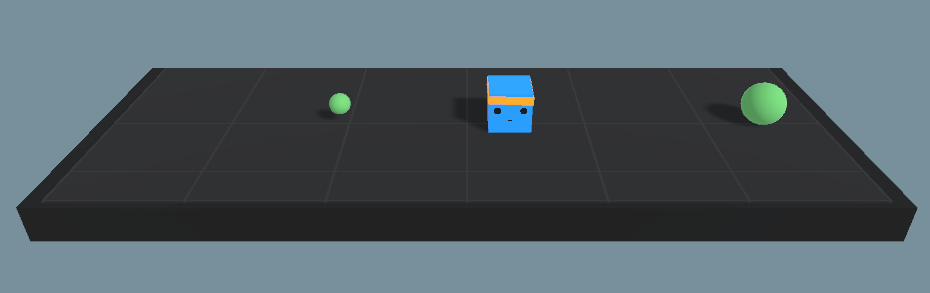
\includegraphics[width=\linewidth,height=\textheight,keepaspectratio]{img/basic_example_environment}
	\caption[Basic Umgebungsbeispiel von ML-Agents]{Screenshot der Basic Beispielumgebung von ML-Agents. Der Agent(blau) muss durch die Bewegung nach links oder rechts ein Ziel(die grünen Sphären) erreichen. Der Kontakt mit der großen Sphäre gibt dabei einen höheren Reward als die kleine Sphäre.}
	\label{fig:basic_example}
\end{figure}
Wenn er beim Ziel ankommt, startet der Prozess von vorn. Die Startposition des Agenten sowie die Position der zwei Ziele ist immer gleich. Die Aufgabe ist sehr simpel und die Handlungen führen ohne Umweg zu einem Reward Signal. Deswegen wird hier der Gamma Wert niedrig gewählt. Das Lernen aus Beispielen ist nur eine Option die möglichst optimalen Werte zu finden. Ein anderer Ansatz wäre über Brute Force verschiedene Parametereinstellungen zu testen und die Ergebnisse zu vergleichen. Aus eigener Erfahrung führen suboptimale Hyperparameterwerte nicht dazu, dass der Agent keinen Fortschritt im Training macht. Meist fällt der Kumulative Reward nur etwas schlechter aus. Anders sieht das bei der Observation, der Reward Vergabe und den Aktionsparametern aus. Diese haben einen deutlich größeren Einfluss auf das Ergebnis und können bei suboptimalen Einstellungen bis zum Fehlschlag des Trainings führen. Mehr dazu im Kapitel Training im Wandel der Zeit.


\subsection{Installation und Nutzung}
Zum Start des Projekts war ML-Agent Release 20 die aktuellste Version, welche am 19.11.2022 veröffentlicht wurde. Der Installationsprozess kann im ML-Agents Github unter Installation\cite{mlagents_install} nachgelesen werden. Um ML-Agents nutzen zu können, sind folgende Schritte notwendig. Die Versionen in der Klammer beschreiben die verwendeten Versionen in diesem Projekt:
\\
\begin{itemize}
	\item Unity 2021.3 oder höher installieren (2021.3.31f1 LTS) 
	\item Python 3.8.13 oder höher installieren (3.9.13)
	\item ML-Agent Github Repository klonen, um die Beispielszenen nutzen zu können (Optional)
	\item Pytorch installieren (1.7.1)
	\item mlagents Python Package installieren (0.30.0)
	\item in Unity im Package Manager:
	\begin{itemize}
		\item Die package.json aus dem com.unity.mlagents Ordner hinzufügen
		\item Die package.json aus dem com.unity.mlagents.extensions Order hinzufügen (Optional)
		\item InputSystems Package im Projekt einbinden (Unity eigenes Package)
	\end{itemize} 	 
	\item Unter <ProjektPfad>Packages/manifest.json “com.unity.nuget.newtonsoft-json“: “3.0.1“ hinzufügen
\end{itemize}
Um zu testen, ob die Installation erfolgreich war, die Windows-Eingabeaufforderung im Projekt öffnen und die virtuelle Umgebung aktivieren. Danach den nächsten Befehl ausführen:
\\
\begin{lstlisting}[language=bash,numbers=none]
	(venv) C:\PfadzumProjekt> mlagents-learn --help
\end{lstlisting}
\noindent
\\
Nun sollten mögliche Befehle, die die mlagents-learn.exe erlaubt dargestellt werden. Da die Übersichtlichkeit in der Eingabeconsole jedoch begrenzt ist, folgen ein paar Befehlsketten, die für dieses Projekt häufig genutzt wurden. Um den Lernprozess zu starten:
\\
\begin{lstlisting}[language=bash,numbers=none]
	(venv) C:\PfadzumProjekt> mlagents-learn
\end{lstlisting}
\noindent
\\
Hierbei wird eine default ID erstellt und danach muss die Szene in Unity gestartet werden und der Agent trainiert mit den Standardwerten der Trainingskonfiguration. Für mehr Kontrolle wird der nachfolgende Befehl verwendet:
\\
\begin{lstlisting}[language=bash,numbers=none]
	(venv) C:\PfadzumProjekt> mlagents-learn config(Position der Datei)\config.yaml(Dateiname) --run-id=ErstesTraining(ID)
\end{lstlisting}
\noindent
\\
Bei dieser Anweisung werden die Trainingskonfigurationen aus der config.yaml geladen und die Ergebnisse des Trainings werden in dem Ordner <ErstesTraining> gespeichert. Ml-Agents bittet noch viele weitere Befehlsketten an. So können alte Trainingsdaten überschreiben oder ein bereits trainiertes Modell verbessert werden, indem man von diesem aus, das Training startet. 